\documentclass[aspectratio=169,10pt]{beamer}

\usetheme{Madrid}
\usecolortheme{default}
\setbeamertemplate{navigation symbols}{}
\setbeamertemplate{footline}[frame number]

\usepackage[T1]{fontenc}
\usepackage[utf8]{inputenc}
\usepackage{amsmath,amssymb}
\usepackage{booktabs}
\usepackage{array}
\usepackage{tikz}
\usetikzlibrary{arrows.meta,positioning,fit,calc,shapes.geometric}
\usepackage{pgfplots}
\pgfplotsset{compat=1.18}

\title[Fairness-Aware Routing]{Fairness-Aware Routing Under Missing Context}
\subtitle{Clinical and Quantum Sequential Decision Systems with MAB, CMAB, and iCMAB Methods}
\author[P. Z. Garcia Bautista]{Piter Z. Garcia Bautista\\Advisors: Daniel Krutz and Travis Desell}
\institute[RIT]{Rochester Institute of Technology\\DSCI 601 -- Applied Data Science I}
\date{Endterm Presentation}

\definecolor{ritorange}{RGB}{247,105,2}
\definecolor{deepblue}{RGB}{31,78,121}
\definecolor{softgreen}{RGB}{72,160,98}
\definecolor{softred}{RGB}{190,75,72}
\definecolor{softgray}{RGB}{245,247,250}
\definecolor{softblue}{RGB}{88,137,174}
\definecolor{softpurple}{RGB}{135,99,171}

\setbeamercolor{title}{fg=deepblue}
\setbeamercolor{frametitle}{fg=deepblue}
\setbeamercolor{structure}{fg=ritorange}

\newcommand{\mab}{\textsc{MAB}}
\newcommand{\cmab}{\textsc{CMAB}}
\newcommand{\icmab}{\textsc{iCMAB}}
\newcommand{\sds}{\textsc{SDS}}
\newcommand{\equitas}{\textsc{EQUITAS}}

\begin{document}

% -----------------------------------------------------------------------------
\begin{frame}
  \titlepage
\end{frame}

% -----------------------------------------------------------------------------
\begin{frame}{15-Minute Presentation Plan}
\begin{enumerate}
    \item Project overview: problem, goal, and contribution.
    \item Updated domain model: clinical and quantum routing as one missing-context problem.
    \item Updated architecture overview and four architecture layer slides.
    \item GitHub code-review break: classes connected to the architecture.
    \item Working demo plan and preliminary results.
    \item Next-semester completion plan.
\end{enumerate}
\vspace{0.5em}
\begin{block}{Rubric alignment}
The deck prioritizes clear figures, background explanation, an updated domain model, layered architecture, code review, and a demo path.
\end{block}
\end{frame}

% -----------------------------------------------------------------------------
\begin{frame}{Project Overview}
\begin{block}{Problem}
Many applied data science systems are \textbf{sequential decision systems}: they route scarce resources under uncertainty, observe only partial feedback, and update future decisions from incomplete evidence.
\end{block}

\begin{columns}[T]
\begin{column}{0.48\textwidth}
\textbf{Clinical routing}
\begin{itemize}
    \item diagnostic tests and retests
    \item triage escalation
    \item model-assisted prioritization
    \item scarce attention during volatile conditions
\end{itemize}
\end{column}
\begin{column}{0.48\textwidth}
\textbf{Quantum routing}
\begin{itemize}
    \item route selection
    \item qubit allocation
    \item entanglement-generation effort
    \item noisy and non-stationary links
\end{itemize}
\end{column}
\end{columns}

\vspace{0.4em}
\alert{Goal:} compare performance and fairness across non-contextual, contextual, and informative contextual bandit policies.
\end{frame}

% -----------------------------------------------------------------------------
\begin{frame}{Clinical Validation Added This Semester}
\begin{block}{New empirical foundation}
The COVID clinical evidence analysis validates two concrete missing-context failures that directly motivate this research.
\end{block}

\begin{columns}[T]
\begin{column}{0.48\textwidth}
\textbf{Case 1: Test allocation}
\begin{itemize}
    \item risk context existed but was not used well
    \item high-SVI, Hispanic, and Black communities were under-served
    \item fair CMAB routing reweights allocation by vulnerability
\end{itemize}
\end{column}
\begin{column}{0.48\textwidth}
\textbf{Case 2: Diagnostic bias}
\begin{itemize}
    \item pulse oximetry missed group-specific calibration context
    \item Black, Hispanic, and Asian patients experienced higher occult hypoxemia
    \item EQUITAS-style mediation can target the ambiguous decision zone
\end{itemize}
\end{column}
\end{columns}

\vspace{0.4em}
\small These cases show that context quality is not just metadata; it affects who receives resources and whose measurements can be trusted.
\end{frame}

% -----------------------------------------------------------------------------
\begin{frame}{Updated Domain Model}
\begin{center}
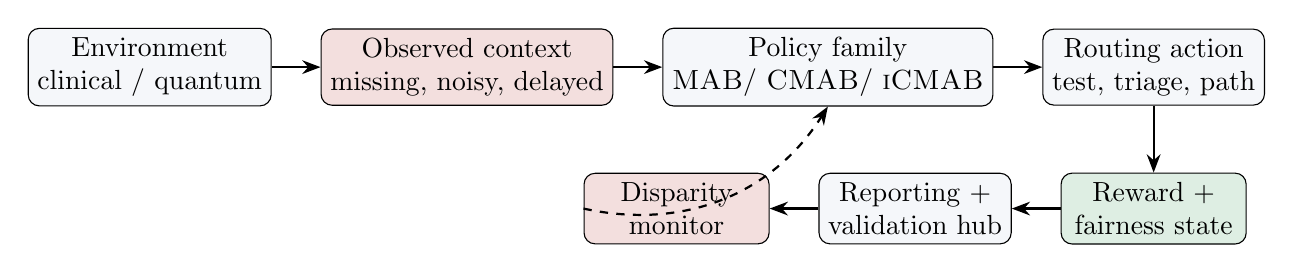
\begin{tikzpicture}[
  node distance=0.9cm,
  box/.style={draw, rounded corners, align=center, minimum width=2.35cm, minimum height=0.75cm, fill=softgray},
  bad/.style={draw, rounded corners, align=center, minimum width=2.35cm, minimum height=0.75cm, fill=softred!18},
  good/.style={draw, rounded corners, align=center, minimum width=2.35cm, minimum height=0.75cm, fill=softgreen!18},
  arr/.style={-{Stealth}, thick}
]
\node[box] (env) {Environment\\clinical / quantum};
\node[bad, right=0.62cm of env] (ctx) {Observed context\\missing, noisy, delayed};
\node[box, right=0.62cm of ctx] (policy) {Policy family\\\mab / \cmab / \icmab};
\node[box, right=0.62cm of policy] (action) {Routing action\\test, triage, path};
\node[good, below=0.85cm of action] (outcome) {Reward +\\fairness state};
\node[box, left=0.62cm of outcome] (report) {Reporting +\\validation hub};
\node[bad, left=0.62cm of report] (harm) {Disparity\\monitor};
\draw[arr] (env) -- (ctx);
\draw[arr] (ctx) -- (policy);
\draw[arr] (policy) -- (action);
\draw[arr] (action) -- (outcome);
\draw[arr] (outcome) -- (report);
\draw[arr] (report) -- (harm);
\draw[arr, dashed] (harm.west) to[bend right=35] (policy.south);
\end{tikzpicture}
\end{center}

\vspace{0.4em}
\begin{itemize}
    \item Multiplicity: one environment produces many contexts; one policy selects one action per round; one action produces one observed reward but many unobserved counterfactuals.
    \item Fairness risk appears when context quality is systematically worse for one group, site, cohort, flow, or route class.
\end{itemize}
\end{frame}

% -----------------------------------------------------------------------------
\begin{frame}{Updated Architecture Overview}
\begin{center}
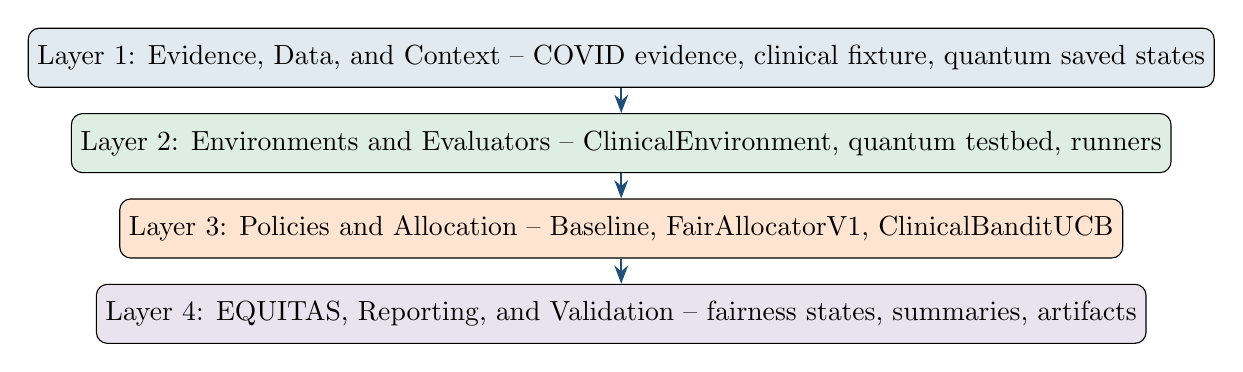
\begin{tikzpicture}[
  layer/.style={draw, rounded corners, align=center, minimum width=10.2cm, minimum height=0.75cm, fill=softgray},
  arr/.style={-{Stealth}, thick, deepblue}
]
\node[layer, fill=softblue!18] (data) {Layer 1: Evidence, Data, and Context -- COVID evidence, clinical fixture, quantum saved states};
\node[layer, fill=softgreen!18, below=0.32cm of data] (env) {Layer 2: Environments and Evaluators -- ClinicalEnvironment, quantum testbed, runners};
\node[layer, fill=ritorange!18, below=0.32cm of env] (policy) {Layer 3: Policies and Allocation -- Baseline, FairAllocatorV1, ClinicalBanditUCB};
\node[layer, fill=softpurple!18, below=0.32cm of policy] (report) {Layer 4: EQUITAS, Reporting, and Validation -- fairness states, summaries, artifacts};
\draw[arr] (data) -- (env);
\draw[arr] (env) -- (policy);
\draw[arr] (policy) -- (report);
\end{tikzpicture}
\end{center}

\vspace{0.4em}
\begin{block}{Design principle}
Low coupling: each layer exposes records/artifacts to the next layer. High cohesion: each layer has one job: context, environment, decision, or validation.
\end{block}
\end{frame}

% -----------------------------------------------------------------------------
\begin{frame}{Architecture Layer 1: Evidence, Data, and Context}
\begin{columns}[T]
\begin{column}{0.48\textwidth}
\textbf{Inputs}
\begin{itemize}
    \item COVID clinical evidence report
    \item clinical synthetic fixture
    \item EQUITAS context fields
    \item quantum legacy saved states
\end{itemize}
\end{column}
\begin{column}{0.48\textwidth}
\textbf{Context fields}
\begin{itemize}
    \item group, site, cohort, service line
    \item test distribution and escalation action
    \item reward, success, latency
    \item route choice, allocator, evaluator state
\end{itemize}
\end{column}
\end{columns}

\vspace{0.6em}
\begin{block}{Why this layer matters}
The COVID evidence makes the clinical context concrete: vulnerability, representation, and measurement quality must be modeled before a fair policy can act.
\end{block}
\end{frame}

% -----------------------------------------------------------------------------
\begin{frame}{Architecture Layer 2: Environments and Evaluators}
\begin{columns}[T]
\begin{column}{0.48\textwidth}
\textbf{Clinical path}
\begin{itemize}
    \item \texttt{ClinicalEnvironment}
    \item \texttt{ClinicalExperimentRunner}
    \item \texttt{ClinicalExperimentEvaluator}
    \item synthetic clinical resource-allocation fixture
\end{itemize}
\end{column}
\begin{column}{0.48\textwidth}
\textbf{Quantum path}
\begin{itemize}
    \item existing quantum-routing testbed
    \item evaluator/runner saved-state conventions
    \item fairness sidecar artifacts
    \item compatibility with legacy experiments
\end{itemize}
\end{column}
\end{columns}

\vspace{0.6em}
\begin{block}{Layer relationship}
The evaluator standardizes outcome records so clinical and quantum runs can be compared through the same reporting and validation surface.
\end{block}
\end{frame}

% -----------------------------------------------------------------------------
\begin{frame}{Architecture Layer 3: Policies and Allocation}
\begin{center}
\begin{tabular}{p{0.24\textwidth}p{0.28\textwidth}p{0.35\textwidth}}
\toprule
Policy family & Decision signal & Fairness risk \\
\midrule
\mab & action history only & can repeat historical allocation patterns \\
\cmab & observed context & can inherit incomplete or biased context \\
\icmab & context + missingness/fairness state & can test whether mediated context reduces harm \\
\bottomrule
\end{tabular}
\end{center}

\vspace{0.6em}
\begin{block}{Clinical model families used in smoke validation}
Oracle, ClinicalBaseline, FairAllocatorV1, and ClinicalBanditUCB.
\end{block}

\begin{equation*}
\text{decision}_t = \arg\max_a \left[\text{utility}_{t,a} - \lambda \cdot \text{expected disparity}_{t,a}\right]
\end{equation*}
\end{frame}

% -----------------------------------------------------------------------------
\begin{frame}{Architecture Layer 4: EQUITAS, Reporting, and Validation}
\begin{columns}[T]
\begin{column}{0.48\textwidth}
\textbf{EQUITAS mediation}
\begin{itemize}
    \item attaches audit/mitigation context
    \item tracks group-conditioned outcomes
    \item separates artifact validation from unvalidated active quantum updates
\end{itemize}
\end{column}
\begin{column}{0.48\textwidth}
\textbf{Reporting layer}
\begin{itemize}
    \item model-stratified fairness summaries
    \item manifest-linked report artifacts
    \item validation hub checks evidence claims
\end{itemize}
\end{column}
\end{columns}

\vspace{0.6em}
\begin{block}{Preliminary framework validation}
The clinical fairness smoke produced 16 fairness states; report generation produced 21 manifest-linked artifacts.
\end{block}
\end{frame}

% -----------------------------------------------------------------------------
\begin{frame}{Clinical Evidence Graph 1: Context-Blind vs Fair Test Routing}
\begin{center}
\begin{tikzpicture}
\begin{axis}[
    ybar,
    width=0.95\textwidth,
    height=0.58\textheight,
    ymin=0,
    ymax=10,
    ylabel={Tests per 1,000 / week},
    symbolic x coords={Hispanic,Black,Mixed,White,Low-Mixed},
    xtick=data,
    x tick label style={rotate=25,anchor=east,font=\scriptsize},
    bar width=7pt,
    legend style={at={(0.5,1.05)},anchor=south,legend columns=2,font=\scriptsize},
    nodes near coords,
    every node near coord/.append style={font=\tiny,rotate=90,anchor=west}
]
\addplot coordinates {(Hispanic,2.1) (Black,2.7) (Mixed,3.1) (White,8.9) (Low-Mixed,7.4)};
\addplot coordinates {(Hispanic,8.4) (Black,7.9) (Mixed,6.8) (White,4.2) (Low-Mixed,3.8)};
\legend{Actual routing,Fair CMAB target}
\end{axis}
\end{tikzpicture}
\end{center}
\vspace{-0.5em}
\small High-SVI Hispanic, Black, and mixed communities receive more tests under context-aware allocation; low-SVI communities receive fewer because their burden index is lower. This turns context into routing evidence rather than post-hoc explanation.
\end{frame}

% -----------------------------------------------------------------------------
\begin{frame}{Clinical Evidence Graph 2: Pulse Oximetry Diagnostic Bias}
\begin{center}
\begin{tikzpicture}
\begin{axis}[
    ybar,
    width=0.95\textwidth,
    height=0.58\textheight,
    ymin=0,
    ymax=32,
    ylabel={Occult hypoxemia rate (\%)},
    symbolic x coords={White,Hispanic,Asian,Black},
    xtick=data,
    bar width=6pt,
    legend style={at={(0.5,1.05)},anchor=south,legend columns=3,font=\scriptsize},
    nodes near coords,
    every node near coord/.append style={font=\tiny,rotate=90,anchor=west}
]
\addplot coordinates {(White,3.6) (Hispanic,5.1) (Asian,6.3) (Black,11.7)};
\addplot coordinates {(White,16.7) (Hispanic,21.4) (Asian,24.1) (Black,29.0)};
\addplot coordinates {(White,14.2) (Hispanic,19.8) (Asian,22.1) (Black,25.6)};
\legend{Sjoding 2020,Fawzy 2022,Fawzy 2023}
\end{axis}
\end{tikzpicture}
\end{center}
\vspace{-0.4em}
\small Across independent studies, Black patients show the highest missed-hypoxemia risk, followed by Asian and Hispanic patients. The same device and threshold produce unequal diagnostic reliability.
\end{frame}

% -----------------------------------------------------------------------------
\begin{frame}{Confusion-Matrix Finding: Diagnostic Reliability Is Unequal}
\begin{columns}[T]
\begin{column}{0.48\textwidth}
\textbf{Baseline single threshold}
\begin{center}
\small
\begin{tabular}{lcc}
\toprule
 & Caught & Missed \\
\midrule
White occult hypoxemia & 96\% & 4\% \\
Black occult hypoxemia & 71\% & 29\% \\
\bottomrule
\end{tabular}
\end{center}
\vspace{0.4em}
\alert{Disparity:} about 25 percentage points in missed hypoxemia.
\end{column}
\begin{column}{0.48\textwidth}
\textbf{Fair CMAB + EQUITAS target}
\begin{center}
\small
\begin{tabular}{lcc}
\toprule
 & Caught & Missed \\
\midrule
White occult hypoxemia & 96\% & 4\% \\
Black occult hypoxemia & 94\% & 6\% \\
\bottomrule
\end{tabular}
\end{center}
\vspace{0.4em}
\alert{Target:} reduce the gap to less than 2 percentage points using targeted threshold/ABG mediation.
\end{column}
\end{columns}

\vspace{0.6em}
\begin{block}{Clinical interpretation}
The fair policy does not need blanket overtesting. It targets the ambiguous SpO$_2$ zone where bias changes treatment eligibility.
\end{block}
\end{frame}

% -----------------------------------------------------------------------------
\begin{frame}{Preliminary Framework Results}
\begin{center}
\begin{tabular}{p{0.43\textwidth}p{0.42\textwidth}}
\toprule
Evidence item & Result \\
\midrule
Clinical embedded path & evaluator, runner, environment, allocator, models, and EQUITAS context run end-to-end \\
Clinical fairness smoke & 16 fairness states across four model families \\
Non-oracle efficiency & FairAllocatorV1: 91.23\%; ClinicalBanditUCB: 84.21\%; ClinicalBaseline: 75.09\% oracle efficiency \\
Reporting layer & 21 manifest-linked artifacts and model-stratified summaries \\
Quantum compatibility & legacy quantum path preserved with fairness sidecar artifacts \\
\bottomrule
\end{tabular}
\end{center}
\vspace{0.3em}
\small Boundary: active fairness-adjusted quantum learning still requires an explicit policy-update mechanism and full validation.
\end{frame}

% -----------------------------------------------------------------------------
\begin{frame}{GitHub Code Review Break}
\begin{block}{Show 2--3 classes not used in the midterm}
During the live code break, open GitHub and connect each class to the architecture diagram.
\end{block}

\begin{center}
\small
\begin{tabular}{p{0.32\textwidth}p{0.48\textwidth}}
\toprule
Class / file to show & Architecture connection \\
\midrule
\texttt{ClinicalExperimentEvaluator} & Layer 2 evaluator orchestration and artifact capture \\
\texttt{ClinicalExperimentRunner} & Layer 2 run execution over seeds, models, and allocations \\
\texttt{FairAllocatorV1} or \texttt{ClinicalBanditUCB} & Layer 3 policy/allocation decision logic \\
\texttt{equitas\_mediator.py} & Layer 4 fairness audit and mitigation context \\
\bottomrule
\end{tabular}
\end{center}

\vspace{0.4em}
\small Mention comments, formatting, and how the classes expose low coupling/high cohesion across layers.
\end{frame}

% -----------------------------------------------------------------------------
\begin{frame}{Working Demo Plan}
\begin{enumerate}
    \item Run the clinical fairness demo or smoke validation notebook.
    \item Show generated fairness states and model-stratified summaries.
    \item Show report artifacts and manifest linkage.
    \item Open the validation hub and point to the five validated evidence claims.
    \item Explain how the COVID clinical evidence can become next-semester executable environments.
\end{enumerate}

\vspace{0.6em}
\begin{block}{Demo objective}
Show that the system is not only conceptual: it runs, records fairness evidence, and produces artifacts connected to the architecture.
\end{block}
\end{frame}

% -----------------------------------------------------------------------------
\begin{frame}{Next Semester: Architecture Completion}
\begin{enumerate}
    \item Convert COVID test allocation and pulse-ox evidence into executable clinical environments.
    \item Add publication-ready figures to the clinical evidence report and presentation pipeline.
    \item Complete active fairness-adjusted quantum policy updates.
    \item Extend validation hub into separate efficiency and fairness hubs.
    \item Build a reporting layer that links framework outputs, validation evidence, and paper claims.
\end{enumerate}
\vspace{0.6em}
\begin{block}{Longer-term goal}
A portal-style reporting surface for queries, experiments, validation, and paper-ready evidence.
\end{block}
\end{frame}

% -----------------------------------------------------------------------------
\begin{frame}{Takeaway}
\begin{block}{Main scientific claim}
Context quality is a fairness variable. Missing, ignored, or biased context can turn partial-feedback learning into repeated allocation harm.
\end{block}

\begin{block}{What was built}
A clinical--quantum evaluation framework that compares performance and fairness across the selected MAB spectrum while preserving reproducible artifacts.
\end{block}

\begin{block}{What the new COVID analysis adds}
COVID test allocation and pulse-ox bias provide real clinical evidence that validates the framework's missing-context harm model.
\end{block}
\end{frame}

% -----------------------------------------------------------------------------
\begin{frame}[allowframebreaks]{Selected References}
\scriptsize
\begin{thebibliography}{99}
\bibitem{bilal2021} Bilal et al. Racial and ethnic inequities in the early distribution of U.S. COVID-19 testing sites. \textit{Social Science \& Medicine}, 2021.
\bibitem{escobar2021} Escobar et al. Addressing COVID-19 testing inequities among underserved communities. 2021.
\bibitem{cdcdisparities} CDC/NCHS. COVID-19 provisional counts: health disparities.
\bibitem{millett2020} Millett et al. Assessing differential impacts of COVID-19 on Black communities. \textit{Annals of Epidemiology}, 2020.
\bibitem{sjoding2020} Sjoding et al. Racial bias in pulse oximetry measurement. \textit{New England Journal of Medicine}, 2020.
\bibitem{fawzy2022} Fawzy et al. Racial and ethnic discrepancy in pulse oximetry and delayed identification of treatment eligibility among patients with COVID-19. \textit{JAMA Internal Medicine}, 2022.
\bibitem{fawzy2023} Fawzy et al. Clinical outcomes associated with overestimation of oxygen saturation by pulse oximetry. \textit{JAMA Network Open}, 2023.
\bibitem{valbuena2022} Valbuena et al. Racial bias and reproducibility in pulse oximetry among medical and surgical inpatients. \textit{BMJ}, 2022.
\bibitem{vaesp2022} VA Evidence Synthesis Program. Differential pulse oximeter accuracy, occult hypoxemia prevalence, and clinical outcomes by race/ethnicity.
\bibitem{garcia2026} Garcia Bautista. DSCI601 project proposal, rough report, architecture, and fairness framework materials.
\end{thebibliography}
\end{frame}

\end{document}
